% Copyright (c) 2008-2009 solvethis
% Copyright (c) 2010-2011 Casper Ti. Vector
% Public domain.



\usepackage{bicaption} \captionsetup[figure][bi-first]{name=图}
\captionsetup[figure][bi-second]{name=Figure} \captionsetup[table][bi-first]{name=表} \captionsetup[table][bi-second]{name=Table}




\documentclass[UTF8]{pkuthss}
% 使得打字机粗体可以被使用。
\usepackage[justification=centering]{caption}
\usepackage{lmodern}
% 产生 originauth.tex 里的 \square。
\usepackage{amssymb}
% 提供 Verbatim 环境和 \VerbatimInput 命令。
\usepackage{fancyvrb}
% 提供数学公式
\usepackage{amsmath}
% 提供theoremstyle
\usepackage{amsthm}
% 提供伪代码
\usepackage{algorithm}  
\usepackage{algpseudocode}
% 提供图片排版
\usepackage{graphicx}
\usepackage{subcaption}
% 提供表格支持
\usepackage{multirow}

\usepackage{verbatim}
% 设定图片路径
\graphicspath{{./img/}}
% pkuthss 文档模版的版本。
\newcommand{\docversion}{v1.3 beta1}

\newcommand{\mycite}[1]
{\citeauthor{#1}\parencite{#1}
}

%
\usepackage{appendix}
% 参考文献格式。
\bibliographystyle{ref/chinesebst-mod}
% 设定文档的基本信息。
\pkuthssinfo{
	cthesisname={研究生毕业论文},ethesisname={Undergraduate Thesis},
	ctitle={机器学习在地震紧急预警系统震级预估中的应用},
	etitle={Application of Machine Learning to Magnitude Estimation in Earthquake Emergency Prediction System},
	cauthor={胡安冬},
	eauthor={Andong Hu},
	studentid={1601210232},
	date={二〇一九年六月},
	school={地球与空间科学学院},
	cmajor={地球物理系},emajor={Geophysics},%direction={震源动力学},
	cmentor={张海明\ 副教授},ementor={Associate Prof.\ Haiming Zhang},
    ckeywords={地震紧急预警; 震级预估; 机器学习; 深度学习},
	ekeywords={Earthquake early warning; Magnitude estimation; Machine learning; Deep learning},
}

% 定义和例子
\theoremstyle{definition}
\newtheorem{example1}{例}
\newtheorem{example2}{例}
\newtheorem{realistic-tra}{定义}
\newtheorem{tra-record}[realistic-tra]{定义}
\newtheorem{tra-data-set}[realistic-tra]{定义}
\newtheorem{same-real-tra}[realistic-tra]{定义}
\newtheorem{tra-matching}[realistic-tra]{定义}

% 算法
\floatname{algorithm}{算法}
\renewcommand{\algorithmicrequire}{\textbf{输入:}}  
\renewcommand{\algorithmicensure}{\textbf{输出:}}  


\begin{document}
	% 以下为正文之前的部分。
	\frontmatter

	% 自动生成标题页。
	\maketitle
	% 版权声明。
	% Copyright (c) 2008-2009 solvethis
% Copyright (c) 2010-2011 Casper Ti. Vector
% All rights reserved.
%
% Redistribution and use in source and binary forms, with or without
% modification, are permitted provided that the following conditions are
% met:
%
% * Redistributions of source code must retain the above copyright notice,
%   this list of conditions and the following disclaimer.
% * Redistributions in binary form must reproduce the above copyright
%   notice, this list of conditions and the following disclaimer in the
%   documentation and/or other materials provided with the distribution.
% * Neither the name of Peking University nor the names of its contributors
%   may be used to endorse or promote products derived from this software
%   without specific prior written permission.
% 
% THIS SOFTWARE IS PROVIDED BY THE COPYRIGHT HOLDERS AND CONTRIBUTORS "AS
% IS" AND ANY EXPRESS OR IMPLIED WARRANTIES, INCLUDING, BUT NOT LIMITED TO,
% THE IMPLIED WARRANTIES OF MERCHANTABILITY AND FITNESS FOR A PARTICULAR
% PURPOSE ARE DISCLAIMED. IN NO EVENT SHALL THE COPYRIGHT HOLDER OR
% CONTRIBUTORS BE LIABLE FOR ANY DIRECT, INDIRECT, INCIDENTAL, SPECIAL,
% EXEMPLARY, OR CONSEQUENTIAL DAMAGES (INCLUDING, BUT NOT LIMITED TO,
% PROCUREMENT OF SUBSTITUTE GOODS OR SERVICES; LOSS OF USE, DATA, OR
% PROFITS; OR BUSINESS INTERRUPTION) HOWEVER CAUSED AND ON ANY THEORY OF
% LIABILITY, WHETHER IN CONTRACT, STRICT LIABILITY, OR TORT (INCLUDING
% NEGLIGENCE OR OTHERWISE) ARISING IN ANY WAY OUT OF THE USE OF THIS
% SOFTWARE, EVEN IF ADVISED OF THE POSSIBILITY OF SUCH DAMAGE.

\chapter*{版权声明}
{
	\zihao{3}\linespread{1.5}\selectfont

	任何收存和保管本论文各种版本的单位和个人,
	未经本论文作者同意,不得将本论文转借他人,
	亦不得随意复制、抄录、拍照或以任何方式传播。
	否则一旦引起有碍作者著作权之问题,将可能承担法律责任。

}


	% 中英文摘要。
	% Copyright (c) 2008-2009 solvethis
% Copyright (c) 2010-2011 Casper Ti. Vector
% Public domain.

\begin{cabstract}
\indent 地震预警是地震减灾工作的重要途径,而震级预估是整个地震紧急预警系统中重要且较为困难的一个环节。目前,世界上多个国家和地区都已建立了各自的地震预警系统,并且形成了特征频率(~$\tau_{p}$~和~$\tau_{c}$~等)相关和特征振幅($P_{d}$等)相关的两类震级紧急预警的方法,但各有局限性。本文在已有的方法和理论基础上,运用机器学习算法,将日本KIK和KNET台网从2015至2017年所记录到的843条地震目录,55426条记录作为全数据集,设计、训练出一套用于常见震级范围的机器学习震级预估模型。与已有方法的预估结果相比,机器学习方法不仅使预估的整体误差和方差下降,同时多台联合评估单一地震事件的截面方差也更低。本研究的结果显示了机器学习算法在震级紧急预估问题上具有较广阔的应用前景,同时也为较为复杂的深度学习类算法框架下端到端模型提供了实践基础和研究可能。
\end{cabstract}

\begin{eabstract}
\indent Earthquake early warning (EEW) is an important way for earthquake disaster reduction, and magnitude estimation is an important and difficult part of the entire EEW system. Nowadays, many countries and regions around the world have established their own EEW systems, and two types of magnitude emergency warning methods, characteristic frequency ((~$\tau_{p}$~and~$\tau_{c}$~, etc.) and characteristic amplitude ($P_{d}$ and others), have be presented. Based on the existing methods and theories, we applied the machine learning algorithm to 55,426 records for 843 earthquakes recorded by the KIK and KNET networks in Japan from 2015 to 2017. By using these records as a full data set, a set of machine learning magnitude prediction models have been designed and trained for common magnitude ranges. Compared with the estimated results of the existing methods, the machine learning method may reduce not only the estimated overall error and variance, but also the cross-sectional variance of multiple joint seismic events. The results of this study show that machine learning algorithm has a broad application prospect in earthquake magnitude emergency estimation, and provides a practical basis and research possibilities for end-to-end model of more complex deep learning algorithm framework as well.



\end{eabstract}


	% 自动生成目录。
	\tableofcontents

	% 以下为正文。
	\mainmatter

	% 绪言。
	% % Copyright (c) 2008-2009 solvethis
% Copyright (c) 2010-2011 Casper Ti. Vector
% Public domain.

\specialchap{绪言}

本文档是“北京大学论文文档模板”的说明文档,
同时也是使用模版的一个示例。

pkuthss 文档模版由三部分构成:
\begin{itemize}
	\item \textbf{pkuthss 文档类}:
		其中进行了学位论文所需要的一些基本的设定,
		主要包括对基本排版格式的设定和提供设置论文信息的命令。
	\item \textbf{pkuthss-extra 宏包}:
		其中实现了学位论文中用户可能较多用到的一些额外功能,
		例如自动在目录中加入参考文献和索引的条目和%
		自动根据用户设定的文档信息对生成的 pdf 的元数据进行设置等。
	\item \textbf{说明(示例)文档}:
		说明文档即本文档,
		在正确安装(见第 \ref{sec:inst} 节)之后应该可以%
		用 \TeX{} 系统提供的 \verb|texdoc| 命令调出:
\begin{Verbatim}[frame=single]
texdoc pkuthss
\end{Verbatim}
		同时,
		本文档的源代码(位于 \verb|doc/| 目录下)%
		也正是用户撰写自己的学位论文时的一个模版:
		用户只需按照模版中的框架修改代码,
		即可写出自己的论文。
\end{itemize}

在此之前,包括 dypang\cite{dypang}、FerretL\cite{FerretL}、%
lwolf\cite{lwolf}、Langpku\cite{Langpku}、%
solvethis\cite{solvethis} 等的数位网友均做过学位论文模板的工作。
本论文模板是 solvethis 的 pkuthss 模板的更新版本,
更新的重点是重构和对新文档类、宏包的支持。

pkuthss 文档模板现在的维护者是 Casper Ti. Vector\footnote%
{\href{CasperVector@gmail.com}{\texttt{CasperVector@gmail.com}}}。


	
	% 各章节。
	% Copyright (c) 2008-2009 solvethis
% Copyright (c) 2010-2011 Casper Ti. Vector
% Public domain.

\chapter{引言}
\section{研究背景}
\indent 我国是遭受地震灾害最为严重的国家之一。在过去的20世纪里,因大陆地震而造成死亡的人数中我国超过60万人,占全球总人数一半以上(金星等, 2003, 2012)。与此同时,随着近海陆地城市化进程的推进,我国60\%的百万人口城市都位于高烈度区域,其中包括全国23个省会城市,地震灾害对这些地区人民的生命和财产构成严重威胁(张红才等, 2012)。为了减少地震灾害造成的生命财产损失,地震预警 (EEW) 系统应运而生。它合理地利用城市和地震源之间的空间关系,同时配合人民群众接受适当的训练以响应地震警报信息,成为减少地震灾害的有效手段 (Allen et al., 2007)。\\
 \indent EEW系统对即将发生强烈震动的城市区域发出预警,在破坏性强的S波部分到达之前通常具有几秒到几十秒的预警时间,这个宝贵的时段可为各种关键设施预设紧急措施:例如紧急制动正在运行的高铁和动车,以避免潜在的脱轨;关闭天然气管道,以最大限度地减少火灾危险;紧急备份与关闭计算机等设施,以避免重要数据库丢失 (Kamigaichi et al., 2009; Allen et al., 2007; Iglesias et al., 2007)。EEW系统包括实时地震定位、实时震级预估、预警目标区烈度估计和预警信息发布四个主要部分。目前已经有成熟的方法进行地震定位和预警信息发布。但作为决定EEW系统好坏的重要环节的实时震级预估,仍存在着诸多难点:首先,大地震震级难以准确测定。较大的地震都是由多个断层破裂组成,单次断层破裂过程也十分复杂;其次,在EEW有时效性的要求下,短时窗内观测到信息少,常用的震级计算方法会在6.5级左右产生明显的震级饱和 (Kanamori et al., 2009);此外,发震断层走向和倾向等参数对地面运动分布也会产生显著影响,但这些震源参数难以实时得到。\\
 \indent 已有的解决方案在很多方面还有待提高。例如,在常见震级范围内漏报和误报情况出现频率较高;为了得到稳定的预估结果,需要的台站较多;仍无法解决震源参数高效实施获得等。单台站震级预估方法因其简单和快速的特点成为当前震级紧急预估的主流方法,但无论是以$\tau_{p}$和$\tau_{c}$ (Nakamura et al., 1993; Kanamori et al., 2005) 为核心的特征频率相关方法,还是以$\mathrm{P}_{\mathrm{d}}$(Wu et al., 2007; Kanamori et al., 2008, 2009) 为核心的振幅相关方法,都只使用了地震台站的垂直分量记录,导致信息极大的浪费。由于两类方法的出发点不同,各自具有一定的局限性,比如$\tau_{c}$类方法在实践中被证实在部分地区效果不好(Horiuchi et al., 2006),而$\mathrm{P}_{\mathrm{d}}$类方法对于长破裂时间的震源更容易震级饱和 (Zollo et al., 2006)。以上研究结果表明,以单一特征为核心的震级预估算法不够强健,促使了相对应的多特征间相容性的研究(张红才等, 2017)。另一方面,如果在EEW系统中加入实时震源参数检测,则会使得准确性与所用时间同时增加 (Heaton et al., 1985; Allen,2006)。例如,在意大利的Preto系统中,预先根据历史地震和对应断层预设数据库,发震后从数据库中自动匹配断层参数 (Weber et al., 2007),但在时效上仍难以达到实时预警的要求。\\
\section{本文研究的意义}
\indent 本文针对EEW系统的实时震级预估问题,采用机器学习类算法解决和优化以上提到的诸多问题。一方面,高密度地震台网记录的地震数据给需求巨量训练数据的机器学习算法提供了训练的可能性;另一方面,机器学习算法可以充分利用台站记录的完整数据,避免了已有算法中只利用单一分量造成的信息浪费。此外,考虑到不同地区断层有不同特点,机器学习算法能自动训练出最适合当地的震级预测模型,这使得模型可以获得最佳适应断层模型和震源参数的影响。本研究显示出新模型预估震级的能力显著优于已有方法,表明机器学习算法在震级紧急预估问题上具有较广阔的应用前景,同时也为较为复杂的深度学习类算法框架下端到端模型提供了实践基础和研究可能。\\
\indent 同时传统震级预估方法对于低信噪比数据的处理能力较低、抗噪声干扰差。以目前两类主流EEWs所使用的震级预估模块的算法特点,都还不能良好处理大型地震后频繁出现的余震。但事实上大型破坏地震之后的余震危害是巨大的,根据中国地震台网中心统计,2008年汶川地震主震发生后的三个月内,共发生6级以上的余震6次,5级至6级的余震30次。(陈九辉等,2009)。这些高强度余震很多时候都会被主震或其他与余震的尾波所干扰,导致使用传统方法在预估余震震级上往往会有较大的偏差。而机器学习CNN类算法在滤波抗噪方面有独特结构带来的优势,即使台站信息被噪音或主震尾波淹没仍可以在一定程度上,从中剥离出需要紧急预估的余震震级。\\

	
\chapter{传统震级预估方法简介}

\section{预估震级的可能性}

\indent 能够由初始破裂信息估计出整个地震的规模是预估震级可行的基本前提。目前学术界对于这个问题仍没有一致性的认识。持否定态度的学者认为破裂过程在时序上是不可预测,即使用已得到的地震台信息只能评估目前的地震释放的能量但不能预估整个断层破裂结束所释放的能量大小(Mori, 1996; Kilb et al, 1999),。但仍有已有多种观点支持根据少量初始信息进行地震震级预估是可行的。首先,在断层初始破裂过程中存在成核震相,而它直接决定了最终破裂的形态 (Ellsworth and Beroza, 1995; 马胜利等, 2002; Dodge et al, 1996);其次,地震产生的P波和S波分别携带不同信息,前者携带着反映断层如何滑动的信息,而后者则携带着地震能量的信息,因此可以分别加以利用,在破坏性较强的S波到来之前,通过P波的特征估计出断层破裂信息 (Beroza et al, 1995)。在这此问题的不断争论中,已有许多研究成果表明在一定的精度要求下是可以做到使用初始破裂信息估计整个地震的规模的 (Allen et al., 2003, 2007; Kanamori et al., 1997, 2005, 2008)。根据不同算法的出发点,大致可以划分为两类,分别是特征频率类方法和特征振幅类方法。\\
\section{特征频率类方法}
\indent 对于估计地震规模的问题,最重要的是确定地震的破裂是否已经停止,或者是仍持续扩展,特征频率类方法就是通过最初的地表震动周期长短来判定地震破裂的持续情况 (Kanamori, 2005; Allen, 2005)。尽管事实上地震破裂的过程往往很复杂,甚至一个大规模地震初始是由一个短周期的初动持续作用引起的,但这并不影响我们从平均意义上研究地震的特征周期(或特征频率)与最终地震规模的关系。\\
\indent Nakamura (1988) 首先提出了利用实时速度记录计算地震动卓越周期的算法,随后经一些研究者拓展形成了对P波拐角频率的特征进行估计的$\tau_{p}^{\max }$方法 (Allen et al, 2003; Olson et al., 2005; Kanamori et al., 1995, 2005)。根据这种方法,\\
\begin{equation}
\tau_{\mathrm{i}}^{\mathrm{p}}=2 \pi \sqrt{\frac{\mathrm{X}_{\mathrm{i}}}{\mathrm{D}_{\mathrm{i}}}}
\end{equation}
式中,$\mathrm{X}_{\mathrm{i}}=\alpha \mathrm{X}_{\mathrm{i}-1}+\mathrm{x}_{\mathrm{i}}^{2}, \mathrm{D}_{\mathrm{i}}=\alpha \mathrm{D}_{\mathrm{i}-1}+\left(\frac{\mathrm{dx}}{\mathrm{dt}}\right)_{\mathrm{i}}^{2}, \tau_{i}^{p}$是i秒时测定的特征周期,$\mathrm{X}_{\mathrm{i}}$是记录的地面运动速度值,$\mathrm{X}_{\mathrm{i}}$是平滑后地面运动速度的平方值,$\alpha$为接近的1的平滑系数 (取值多为0.999)。$\tau_{p}^{\max}$台站P波触发后的若干秒后,该迭代序列中的最大值。美国著名的ElamrS系统就采取$\tau_{p}^{\max }$法进行的震级预估 (Allen et al, 1996)。ElamrS系统实践表明,$\tau_{p}^{\max}$台站数量要求较高,多台站联合预估结果的误差在台站数量较少的情况下与其数量近似呈现线性关系,5个台站平均误差约为±0.70,10个台站误差下降至±0.35 (Kanamori et al., 2005)。$\tau_{p}^{\max}$法的准确和稳定性同时还受台站记录的采样率影响,与数据预处理方式密切相关,选用不同滤波器或滤波时窗都会对特征周期的计算结果产生较大影响。例如当选用较大的高频截止频率对记录低通滤波处理后,特征周期计算结果会明显偏小。Allen (2003, 2007)在后续的一系列的工作中对$\tau_{p}^{\max}$法进行可改进,在预估震级前给出预分类假设。在不同的预分类情况下使用不同的滤波方式,以得到该情形相应的震级并基于多种情景假设共同预估出震级。\\
\indent Kanamori(2005)随后提出了一种对$\tau_{p}^{\max}$改进的捕捉特征周期计算方法,称为$\tau_{\mathrm{c}}$方法,计算方法如下:\\
\begin{equation}
\mathrm{r}=\frac{\mathlarger{\int}_{0}^{\tau_{0}} \dot{\mathrm{u}}^{2}(\mathrm{t}) \mathrm{dt}}{\mathlarger{\int}_{0}^{\tau_{0}} \mathrm{u}^{2}(\mathrm{t}) \mathrm{dt}}
\end{equation}
\begin{equation}
\tau_{\mathrm{c}}=\frac{2 \pi}{\sqrt{\mathrm{r}}}
\end{equation}
其中u和$\dot{u}$̇是地震台站垂直分量记录的地表位移和速度,所计算的系数r是对特征频率平方的一种估计。式中积分区间为$\left[0, \tau_{0}\right]$,代表台站触发P波记录后$\tau_{0}$秒内的记录。研究表明,在大多数情况下$\tau_{0}$设置为3s即可(Wu and Kanamori, 2005a, 2005b, 2007)。使用Parseval定理可以将(2.2)和(2.3)式改写为:
\begin{figure}[!h] 
\centering 
 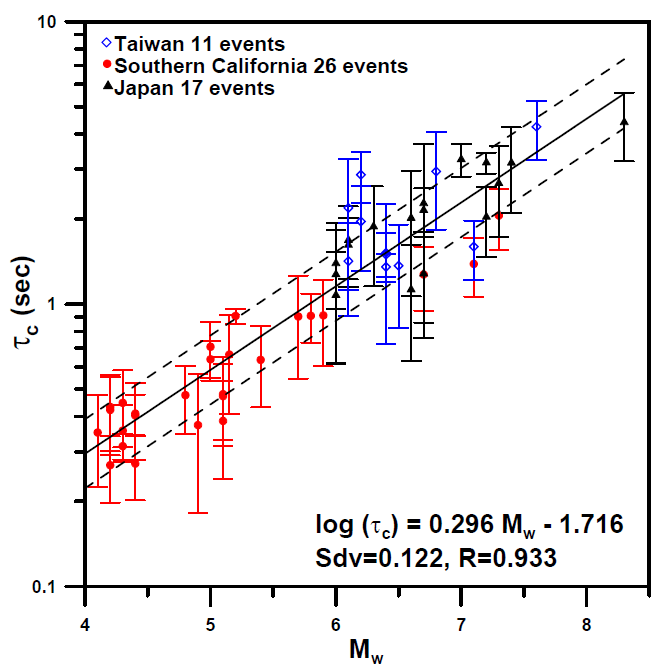
\includegraphics[width=0.7\linewidth]{img/kanamori2008_taoc.jpg} 
 \renewcommand{\figurename}{图} 
\caption{Kanamori et al. (2008)对于$\tau_{\mathrm{c}}$方法的研究(共使用54个地震事件)} 
%英文标题begin 
\addtocounter{figure}{-1} \vspace{-5pt} 
%\SetEnglishCaption 
\renewcommand{\figurename}{Fig} 
\caption{Kanamori et al. (2008) Study of the $\tau_{\mathrm{c}}$ method (using a total of 54 seismic events)} 
\renewcommand{\figurename}{图} 
%英文标题end 
\label{fig:network-device-influence.png} 
\end{figure}

\begin{equation}
\mathrm{r}=\frac{4 \pi^{2} \int_{0}^{\infty} f^{2}|\widehat{u}(f)|^{2} d f}{\int_{0}^{\infty}|a(f)|^{2} d f}=4 \pi^{2}\left\langle f^{2}\right\rangle
\end{equation}
\begin{equation}
\tau_{c}=\frac{1}{\sqrt{\left\langle f^{2}\right\rangle}}=\frac{2 \pi}{\sqrt{r}}
\end{equation}
其中$\widehat{u}(f)$为位移记录u(t)的频谱,$\left\langle f^{2}\right\rangle$为以$|\hat{u}(f)|^{2}$加权的频率平方平均值。在此定义下,$\tau_{\mathrm{c}}$即为P波初至时段内地震波的主要周期,也即是对P拐角频率的另一种特征估计,故可以用于估计断层破裂情况。与$\tau_{p}^{\max}$相比,$\tau_{\mathrm{c}}$方法更为稳定,需要更少的台站就可以得到稳定预测结果。在实践中,$\tau_{\mathrm{c}}$对于不同地区的差异性也更小 (Wu et al., 2005, 2008),在中国台湾、美国加州、日本地区都能得到一致结果。\\

\section{特征幅值类方法}

 \indent 使用地震台站记录的特征幅值预估震级的方式表面上与传统的震后震级确定的方法很接近,但从工作原理上来看两者有重要区别。由于时效性需求,特征幅值类方法要求使用短时间少量信息提取出特征幅值以预估震级,而震后确定工作更多完成的是标定工作。地震波在地球介质传播过程中,震动幅值会随着震中距的增大而衰减,特征幅值类的预估过程中就是利用了这种衰减关系。相同情况下由位移信息提取的幅值参数所得到的预估震级结果优于由速度、加速度信息所得的 (马强等, 2008),而台站记录中垂直向分量中的P波最为发育,故此类方法基本选择从台站垂直向记录中提取位移特征幅值。\\
 \indent 特征幅值类算法中,$\mathrm{P}_{\mathrm{d}}$方法最优。$\mathrm{P}_{\mathrm{d}}$一般定义为,台站垂直分量的位移记录在P波触发后3s时窗采用2阶高通巴特沃斯滤波器(常见低频截止频率为0.075Hz)滤波后的位移最大值(Wu et al., 2007)。$\mathrm{P}_{\mathrm{d}}$参数不仅与震级有关,也与地震动速度峰值PGV和加速度峰值PGA之间有相关性。$\mathrm{P}_{\mathrm{d}}$参数比较稳定,对地区差异性不敏感,经过震中距R修正后的规律在不同国家和地区都得到了统一验证,因此$\mathrm{P}_{\mathrm{d}}$参数可以作为预警目标区地震烈度估计的有利判据。$\mathrm{P}_{\mathrm{d}}$与$\mathrm{M}_{\mathrm{w}}$、PGV的关系可以表示为\\
\begin{equation}
\log \left(\mathrm{P}_{\mathrm{d}}\right)=\mathrm{A}_{1}+\mathrm{A}_{2} \mathrm{M}_{\mathrm{W}}+\mathrm{A}_{3} \log (\mathrm{R})
\end{equation}
\begin{equation}
\log \left(\mathrm{P}_{\mathrm{d}}\right)=\mathrm{B}_{1}+\mathrm{B}_{2} \log (\mathrm{PGV})
\end{equation}
 其中MW为矩震级,$\mathrm{A}_{\mathrm{i}}$和$\mathrm{B}_{\mathrm{i}}$分别为在局部地区$\mathrm{P}_{\mathrm{d}}$与$\mathrm{M}_{\mathrm{w}}$和$\mathrm{P}_{\mathrm{d}}$线性关系系数。$\mathrm{P}_{\mathrm{d}}$方法的劣势在于存在震级饱和现象。若设置时间窗长度为3s时,$\mathrm{P}_{\mathrm{d}}$方法的饱和震级约为6.5级,而当时间窗长度达到4s时饱和震级可以提高至7.0级 (Zollo et al., 2006)。\\
	% Copyright (c) 2008-2009 solvethis
% Copyright (c) 2010-2011 Casper Ti. Vector
% Public domain.

\chapter{机器学习类震级预估算法}
\indent 随着大数据时代到来,现代生产建设中设备不断电子化使得数据量呈指数增长,同时电子计算机硬件性能不断突破、计算能力不断提高,这些变化都给人工智能领域快速发展提供了优渥的土壤。例如具体到人工智能中的深度学习算法,过去受限于数据量和计算能力导致应用范围有限进展缓慢,而目前随着各领域大数据的帮助和图形处理器的广泛使用已经开始应用于各个各行各业。相比传统的统计学习方法,机器学习类方法的设计更加复杂多样,原理上提供了无需手动进行特征工程而是通过模型深层结构的学习到数据内在规律的可能性。\\
\indent 在过去90年代中,止人工智能与地球物理学的联合交叉应用仍处于起步阶段。很多学者对于机器学习算法拾取P波初至的问题进行了深入的探索(Murat et al., 1993;D.McCormack et al., 1993;), 但受限于当时算法和数据的局限大部分研究都处于尝试阶段。随着宽频带地震仪的普及与全球各地高密度台网的出现,台站地震数据数量和质量双双大幅提升,地球物理学领域的人工智能方法不断前进获得井喷式的发展。CNN模型在地下结构反演方向得到优秀的应用(Das et al., 1993),而端到端训练的CNN、DnCNN模型在地震数据的噪音压制方面的优势也不断被挖掘(王钰清等, 2019),例如在数据增广插值(Wang et al., 1993)、微地震识别和地震事件检测(John et al., 2018)等地球物理与人工智能交叉应用的其他方向也有长足发展。\\
\section{神经网络类算法}
\indent 考虑到特征频率和特征幅值两类算法的局限性,本文首先选取了机器学习中神经网络类算法进行对传统方法进行改进。神经元是构成神经网络最基础的单元,它的结构可抽象成如下图1所示的简单数学模型 (McCulloch and Pitts, 1943),即“M-P神经元模型”。在这个模型中,一个神经元接收到来自n个其他神经元传递过来的输入信号$\mathrm{X}_{\mathrm{i}}$,这些输入信号通过带权重$\mathrm{w}_{\mathrm{i}}$的连接方式进行传递,并将神经元接收到的总输入值$\sum_{i=1}^{n} W_{i} x_{i}$将与神经元的阀值θ进行比较,然后通过“激活函数”处理以产生神经元的输出,这样就完成一个神经元的运算过程。把许多个这样的神经元按一定的层次结构连接起来,就得到各种结构的神经网络。\\
\begin{figure}[!h] 
\centering 
 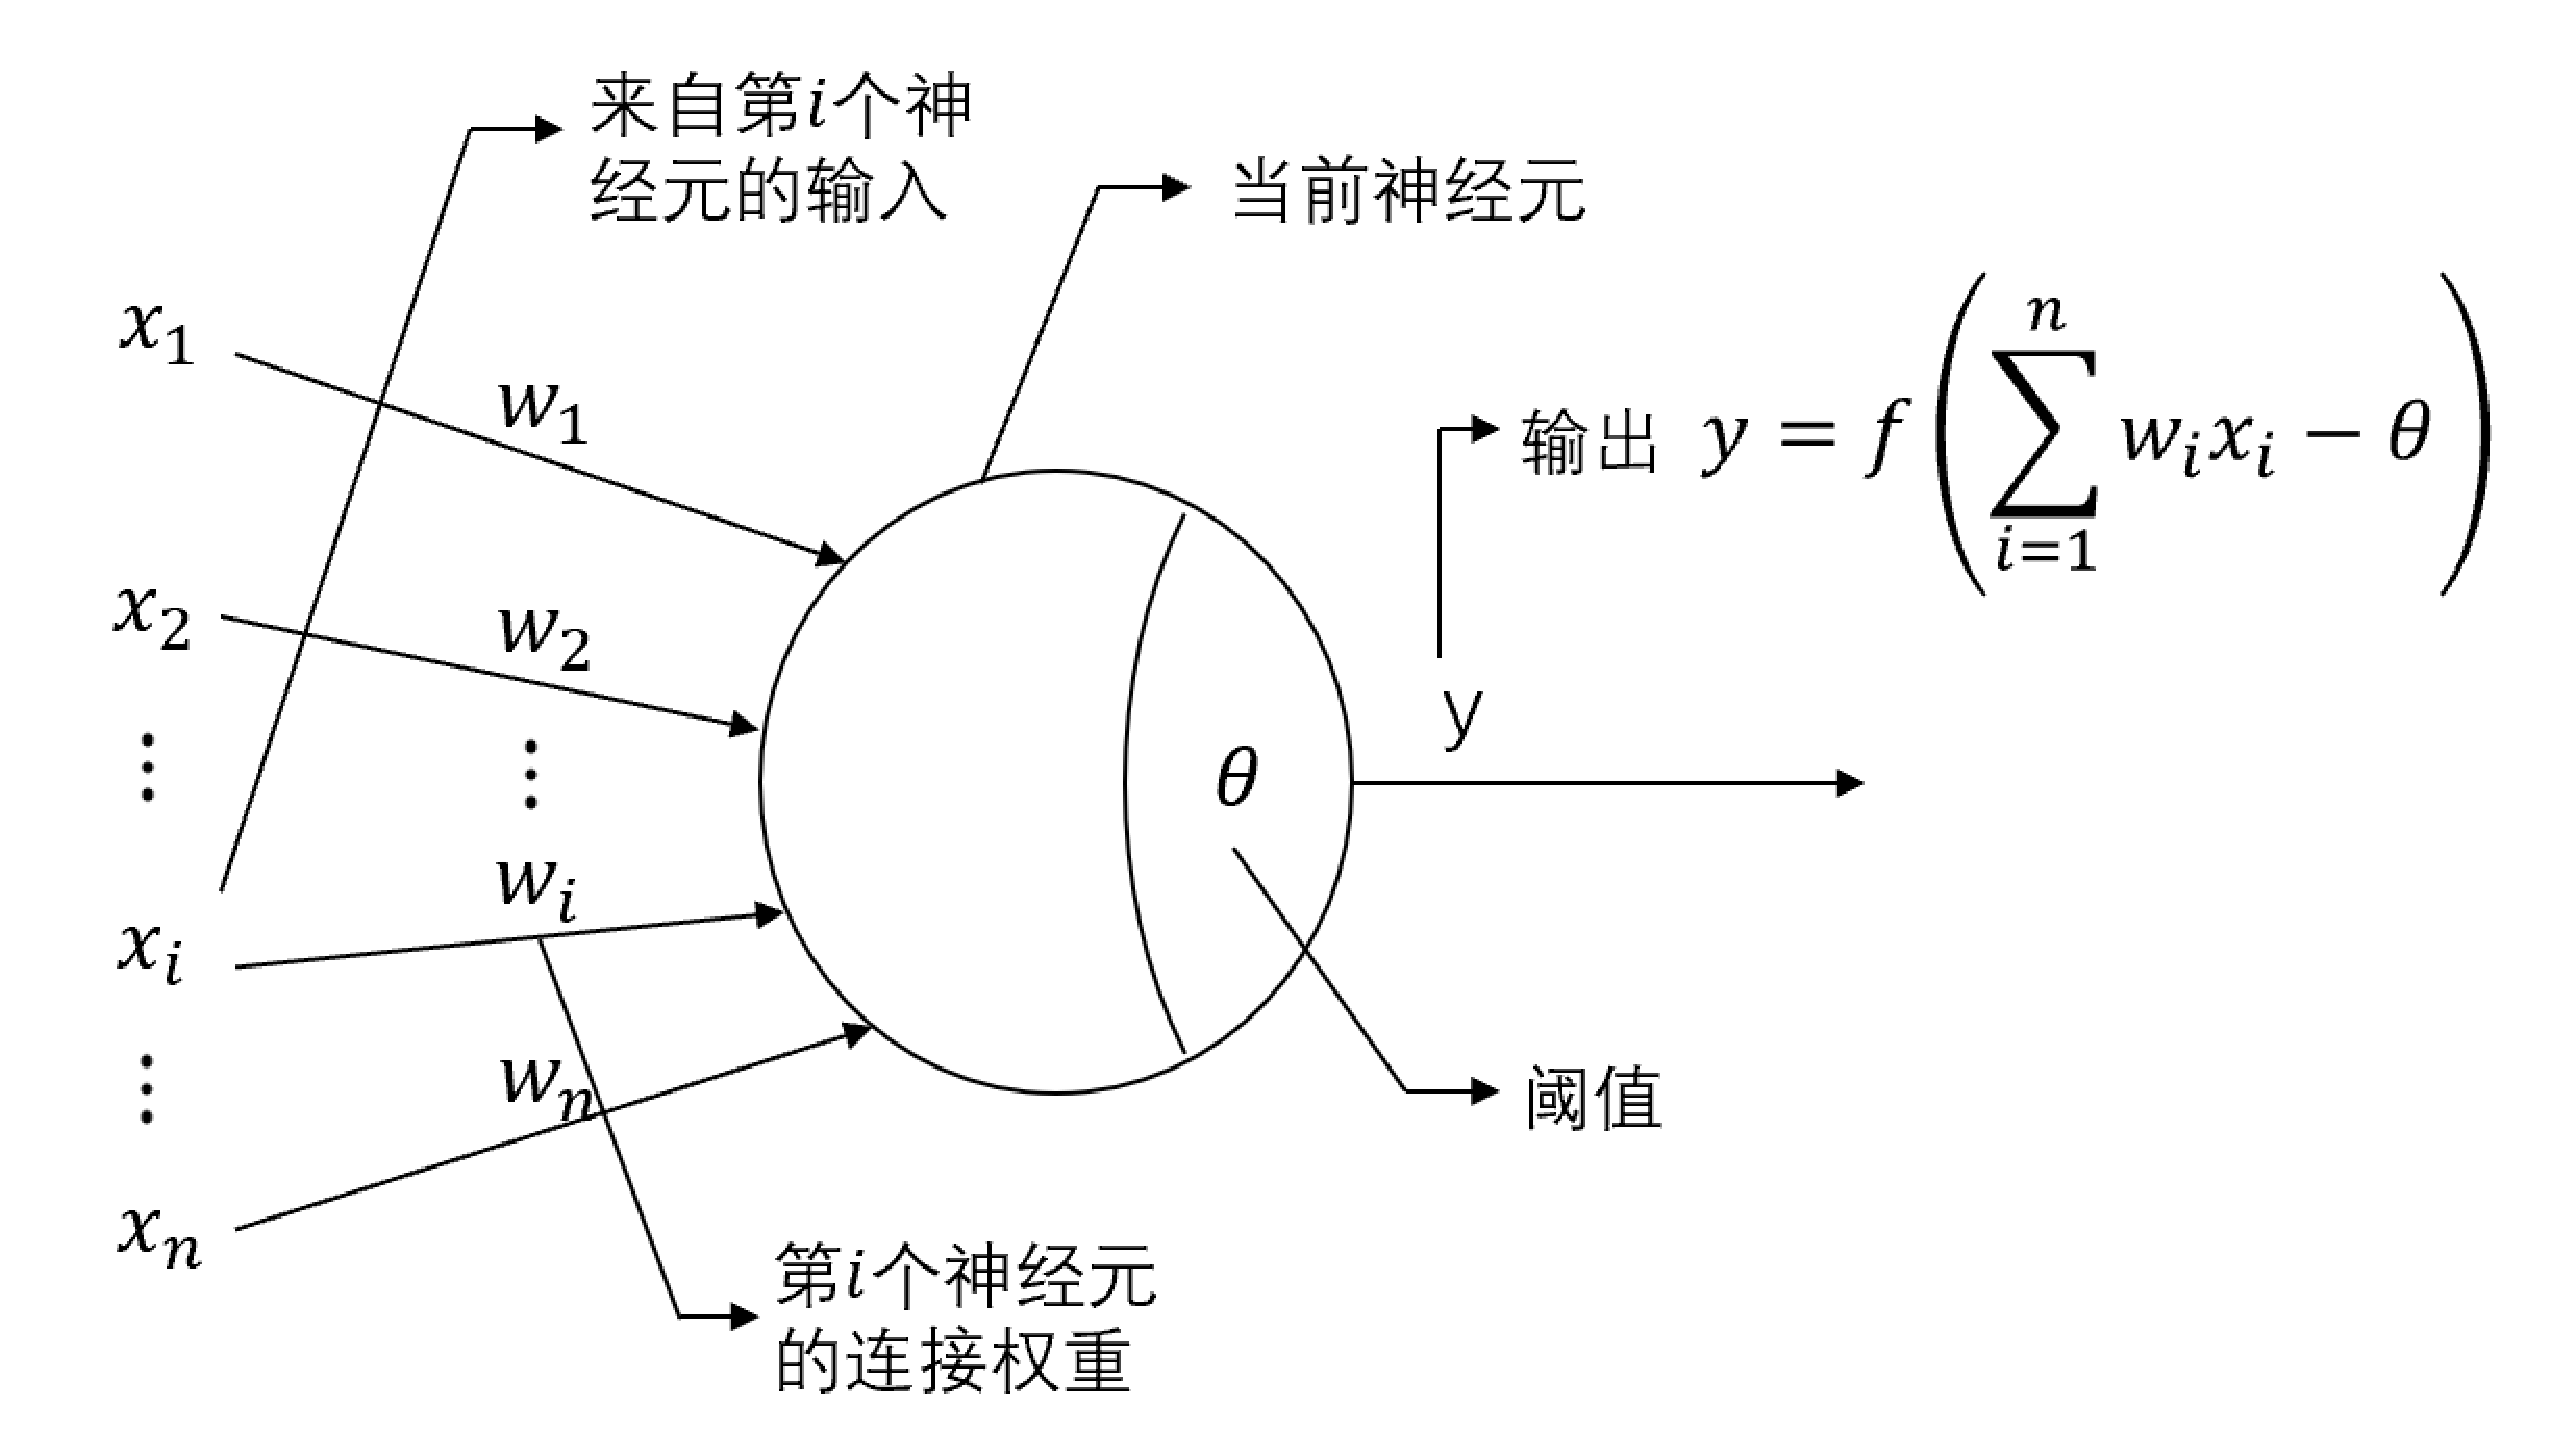
\includegraphics[width=0.75\linewidth]{img/mp.eps} 
 \renewcommand{\figurename}{图} 
\caption{M-P神经元模型示意图} 
%英文标题begin 
\addtocounter{figure}{-1} \vspace{-5pt} 
%\SetEnglishCaption 
\renewcommand{\figurename}{Fig} 
\caption{M-P Neurons model schematic} 
\renewcommand{\figurename}{图} 
%英文标题end 
\label{fig:network-device-influence.png} 
\end{figure}
\section{两类模型的设计}
\indent 我们按照不同训练思路设计出两种神经网络模型用以预估震级。损失函数是机器学习模型效果的评判标准,通过调整模型参数来最小化损失函数以达到优化模型性能的目的。本研究的两种模型的训练目标都按(3.1)式设置,使用平方误差作为损失函数L。将模型设置为回归问题进行训练,通过(3.1)式使用BP算法采用梯度下降的方式最小化损失函数以得到优化的神经网络权值$\theta^{*}$(Werbos, 1974; Rumelhart et al., 1986a,b),其中$\mathrm{W}_{\mathrm{i}}$代表第i个隐藏层。同时如下(3.2)式加入网络权值的
$\mathrm{L}_{1}$、$\mathrm{L}_{2}$范数的进行正则约束以防止过拟合。\\
\begin{equation}
\theta^{*}=\arg \min \frac{1}{N} \sum_{i=1}^{N} L\left(y_{i}, f\left(x_{i} ; \theta_{i}\right)\right)+\sum_{q=1}^{z} \Phi\left(W_{q}\right)
\end{equation}
\begin{equation}
\left\{\begin{array}{c}{L\left(y_{i}, f\left(x_{i}\right)\right)=\left|y_{i}-f\left(x_{i}\right)\right|^{2}} \\ {\Phi\left(W_{q}\right)=\lambda_{1}\left|W_{q}\right|+\lambda_{2} W_{q}^{2}}\end{array}\right.
\end{equation}
其中arg⁡min算符定义为$\theta^{*}=\arg \min f(\theta)$下
,使$f(\theta)$达到最小值的$\theta$值,N为采用mini-batch方式每次训练抽样数量的大小,z代表隐藏的层数。\\
\subsection{NN模型的设计}
\indent NN模型结构如图2所示,也被称为多层感知机(Multilayer-Perceptrion)模型。整体框架为全连接神经网络,相邻层间的所有神经都互相连接,隐藏层间连接方式为下(3.3)和(3.4)式,
\begin{equation}
\mathrm{Z}_{\mathrm{c}}^{i}=\sigma\left(b_{c}^{i}+\sum_{c^{\prime}=1}^{c_{i}} Z_{C^{\prime}}^{i-1} \cdot W_{C C^{\prime}}^{i}\right)
\end{equation}
\begin{equation}
\sigma(x)=\max (0, x)
\end{equation}
其中下角标C,$C^{\prime}$代表了输出层和输入层,上角标i代表第i个隐藏层。激活函数使用(3.4)式中所示的以0为分界的分段函数ReLU(Alex et al., 2012)。当此激活函数接收到前一隐层小于0的输入时输出0,而当接收到大于0的隐藏层输入时不做处理直接作为输出。NN模型以特征频率类方法的思想为基础,但区别于$\tau_{\mathrm{C}}$方法只使用垂直分量的信息,此NN神经网络的使用台站记录的全三分量信息,以期望得到不同分量联合与破裂规模的内在关系。\\
\indent 将3s时窗内的三分量傅里叶变换下的频谱信息并列为一维向量作为模型输入,直接将预估的震级结果设计为模型输出。整个NN模型共有7层神经网络,除去首尾的输入、输出层外共设置5个隐藏层以增强网络的非线性表达能力。根据Hinton(2012a,2012b)和Alex(2012)等人对于机器学习算法过拟合和避免网络陷入局部最优的相关研究,我们在第1和第3隐层后连接Dropout层以防止过拟合,同时加快有效训练速率。\\
\begin{figure}[!h] 
\centering 
 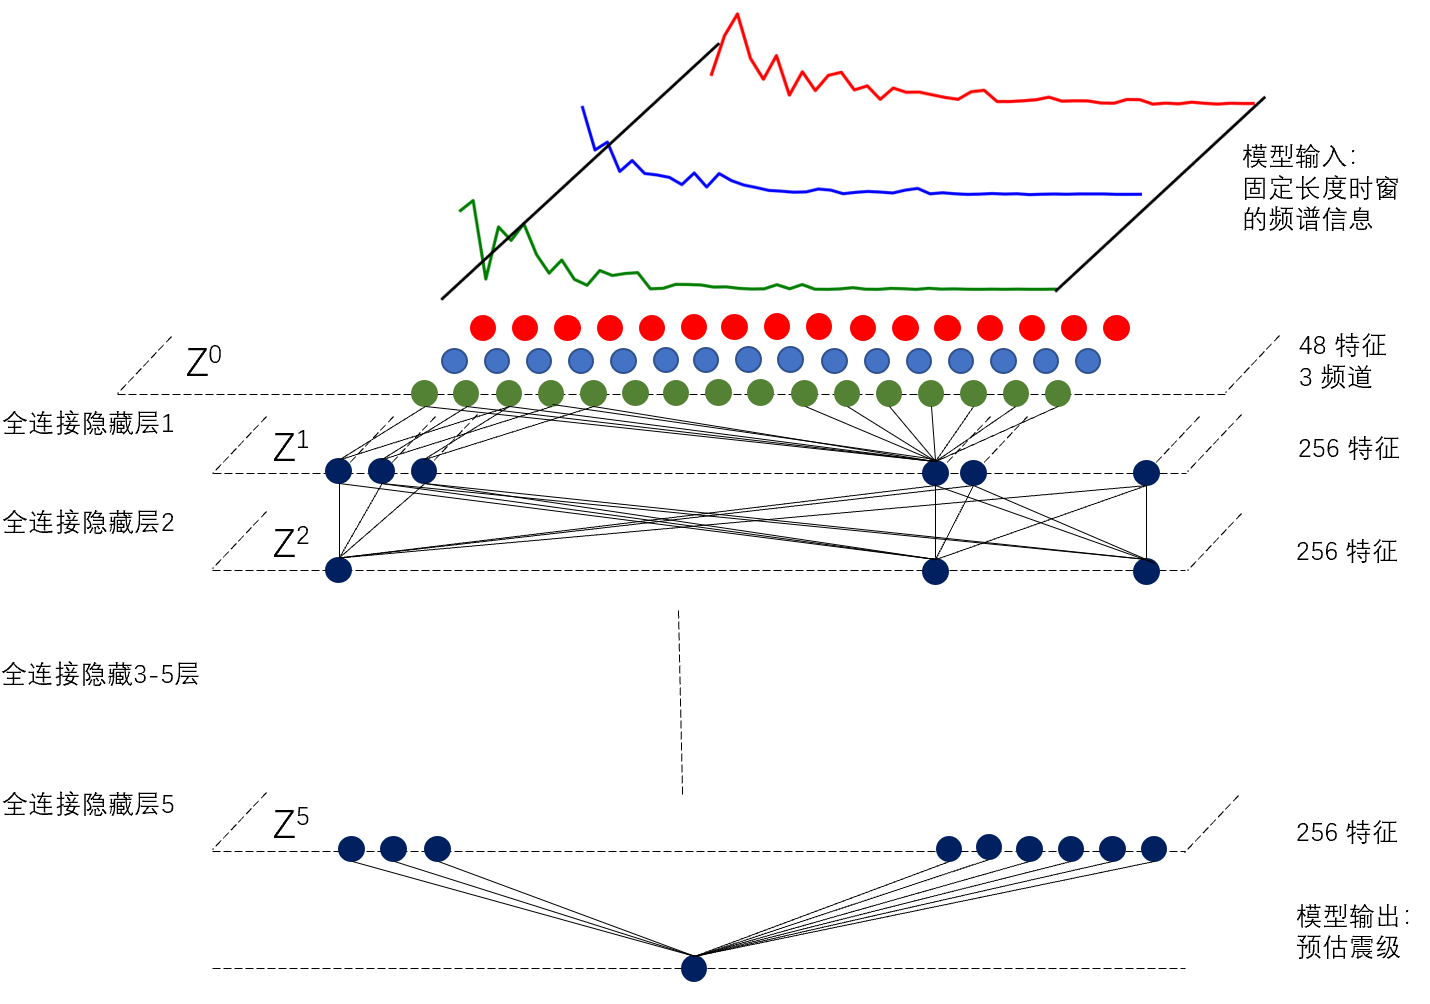
\includegraphics[width=0.99\linewidth]{img/NN.png} 
 \renewcommand{\figurename}{图} 
\caption{NN神经网络结构示意图} 
%英文标题begin 
\addtocounter{figure}{-1} \vspace{-5pt} 
%\SetEnglishCaption 
\renewcommand{\figurename}{Fig} 
\caption{NN neural network mechanism diagram} 
\renewcommand{\figurename}{图} 
%英文标题end 
\label{fig:network-device-influence.png} 
\end{figure}
\subsection{CNN模型的设计}
\indent 卷积神经网络(Convolutional Neural Networks)模型(Fukushima K,1979)是一类包含卷积计算且具有深度结构的前馈神经网络,在图像识别、语音识别等诸多领域有着非常广泛应用的深度学习模型。以常见的卷积神经网络应用场景中数据的结构和特征来看,无论是单通道的音频信息、时频信号还是图像处理问题中三通道RGB图像输入都与地震台站三分量地震波形数据有着很大的相似性。这些问题上的相似性使得CNN网络结构在处理地球物理学问题上有着得天独厚的优势,本文研究模型以图像分类中常用的LeNet-5 模型(LeCun Y et al.,1998)为基础框架,并根据Masaru(2019)等人关于地震问题特性进行SRSpec-CNN模型的相关研究 ,设计出针对三分量地震波形数据特点的震级紧急预估结构。\\
\indent 在传统方法和上节中所提到的NN方法都没有利用到台站信息时序的特点。例如以$\mathbf{\tau}_{\mathrm{c}}$为核心的震级预估算法是直接利用截断时间内频率域特点,并没有利用到台站记录数据中所拥有的P波时间结构特征。3.2.1节所描述的NN方法也只是利用神经网络算法所拥有的强大表达能力,从频率域数据中挖掘出更多描述能量的特征用以进行震级预估。而本章节所设计的CNN震级预估模型中输入信息为如图3.3所示的拥有时间结构小波信号,这就提供了利用P波时间结构特点的可能性。\\
\indent 小波变换是20世纪80年代由石油信号处理工程师J.Morlet提出并发展起来的一种变换分析的新方法(J.Morlet et al., 1983,1984,1985)。小波变换作为时频变换方法,在短时傅里叶变化(Short-time Fourier Transform,STFT)的基础上更多体现出能良好时频局部化特性。在此之前的时频分析领域最为主流的短时傅里叶变换,主体思想为将整个时间域过程分解成在时间上等长的多个小过程分段进行傅里叶变换,并假设这些短过程间的信号是平稳并且相似的。但真实世界中的很多信号都是非平稳的,例如地震台站所记录到的地震波信号
此拥有不同时间的不同特征。方法提出以来
具更是有可以同时在时间域和频率域分析的特点,在地震数据处理中有着重
要的应用,近年来也已经被应用于震相拾取工作中(Chakraborty A, Okaya D. ,1995;
刘希强, 周蕙兰, 沈萍,等, 2000)。
\begin{equation}
C W T_{(a, b)}\{s(t)\}=|a|^{-1 / 2} \int_{-\infty}^{\infty} s(t) \psi^{*}(t-b) / a d t
\end{equation}


\begin{figure}[h] 
\centering 
 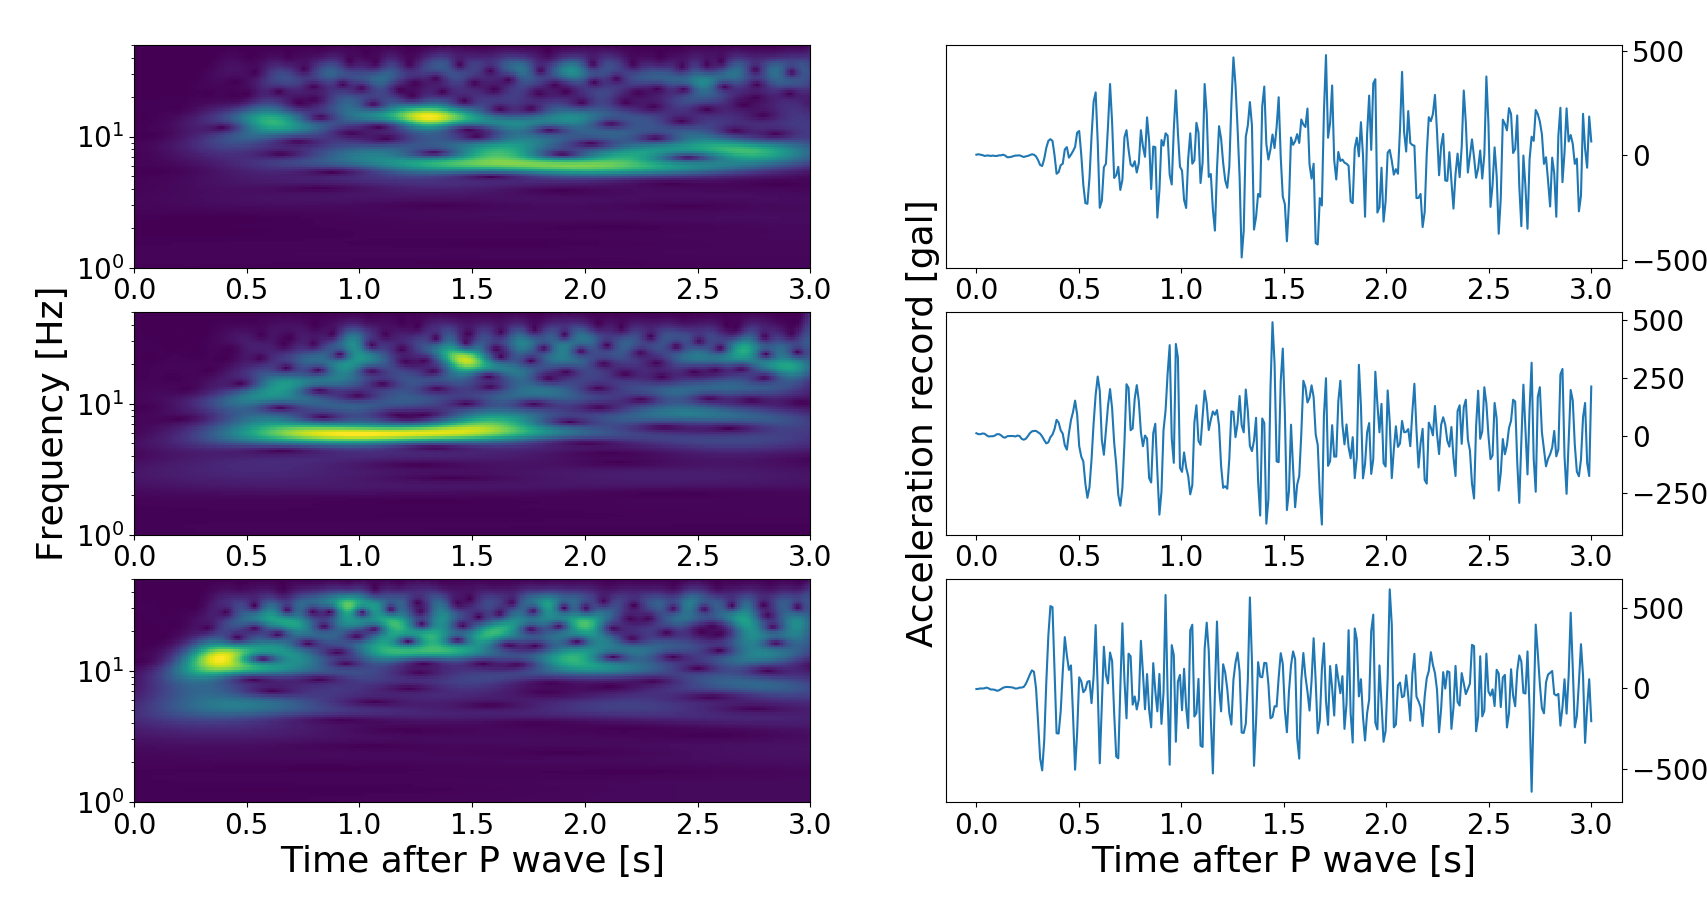
\includegraphics[width=0.99\linewidth]{img/wavelet.jpg} 
 \renewcommand{\figurename}{图} 
\caption{CNN深度神经网络输入信号:P波初到后三秒垂向小波时频谱图} 
%英文标题begin 
\addtocounter{figure}{-1} \vspace{-5pt} 
%\SetEnglishCaption 
\renewcommand{\figurename}{Fig} 
\caption{CNN deep neural network input signal: spectrum of the vertical wavelet when the P wave arrives for three seconds} 
\renewcommand{\figurename}{图} 
%英文标题end 
\label{fig:network-device-influence.png} 
\end{figure}
\indent CNN模型结构如图3所示,整体框架为CNN卷积神经网络。与NN模型相同,使用ReLU作为激活函数,使用全三分量信息,并仍以预估的震级结果作为模型输出。不同的是,CNN模型将3s时窗内的加速度记录处理为三维张量(tensor)作为模型输入,全网络共设置8层卷积层且无池化层设置。卷积层采取小卷积核进行卷积计算,同时采用2个步长的卷积时窗移动以帮助卷积核降采样。卷积隐藏层的运算方式见(10)式。在第8层卷积层后,将所有特征重排列与台站和震中经纬深度信息一同并列后,进行全连接运算输出。考虑到深度学习卓越的表达能力,$\mathbf{\tau}_{\mathrm{c}}$方法中傅里叶变换的预处理是很容易被卷积神经网络完成的,并且还会有更多其他的特征被卷积核提取。\\
\indent 考虑到模型输入的信息量和CNN网络的表达能力,理论上此模型至少可达到$\mathbf{\tau}_{\mathrm{c}}$和$P_{d}$方法的效果。如图3所示,此模型与NN模型相比还引入了台站和震源的位置信息。并且不同于$P_{d}$方法中相对量震中距离的使用,引入台站和震源的坐标信息还在一定程度上可以帮助模型完成区域断层信息、地球介质模型记录,使模型作为区域震级预估方法有更出色的表现。此深度学习模型对原始输入信号进行逐层加工,从而把初始的、与输出目标之间联系不太密切的输入表示,转化成与输出联系更为密切的新表示方式,使得原本难以完成的任务成为可能(对比于NN模型频谱信息输入和最后输出间的映射)。\\
\indent CNN模型端到端的模型设置导致其训练难度更大,也意味着就需要更多的训练数据,由于目前数据量不足暂时还未对CNN模型完成训练。\\
\begin{figure}[h] 
\centering 
 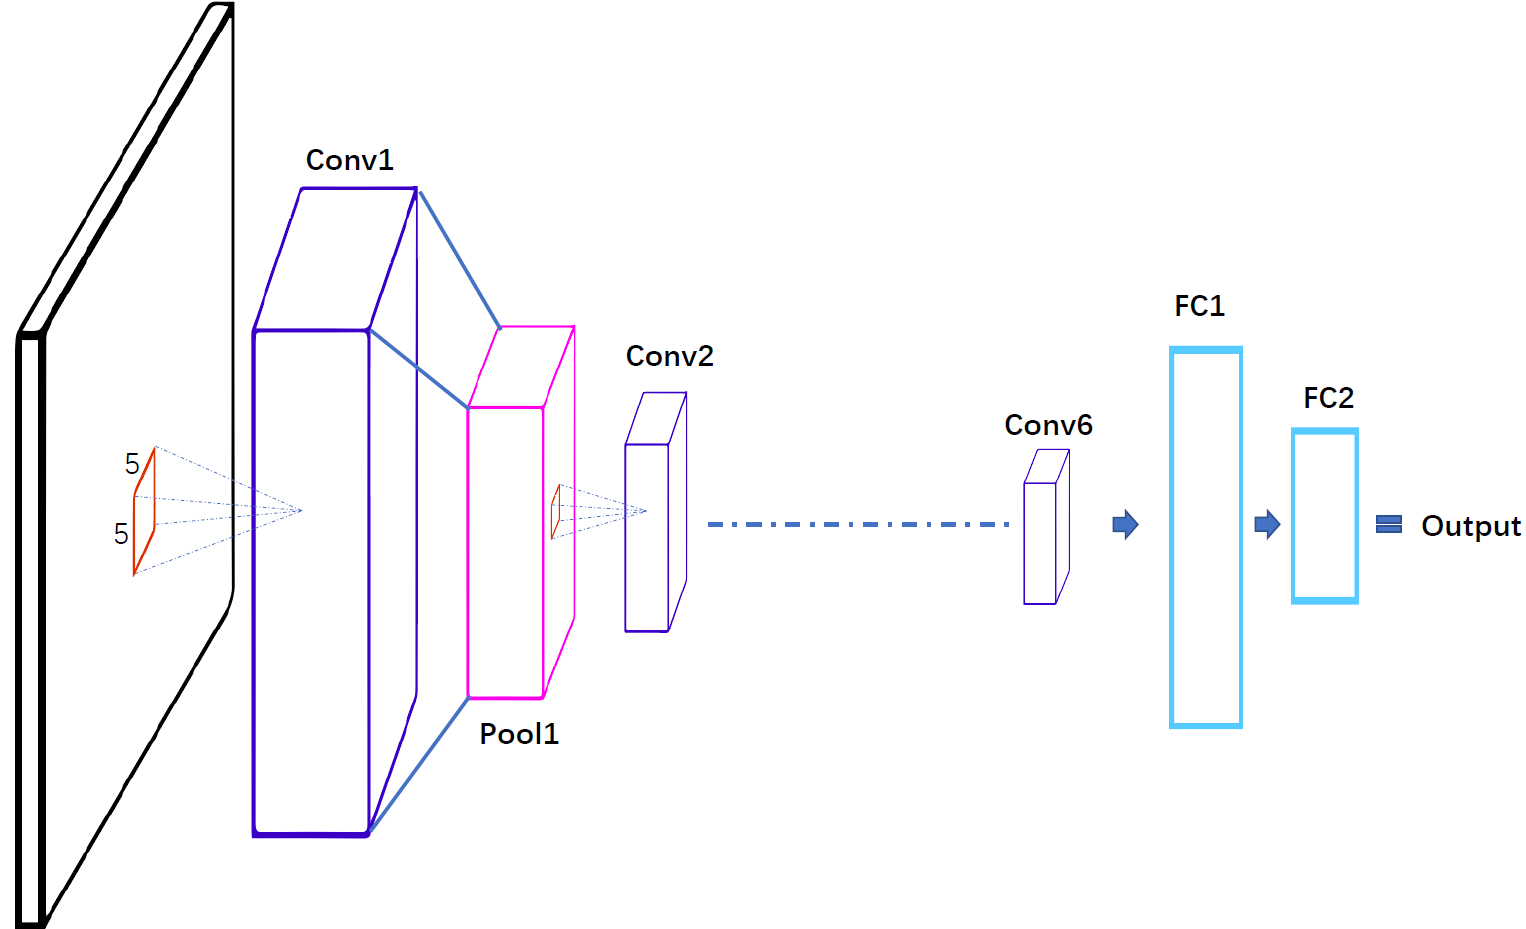
\includegraphics[width=0.99\linewidth]{img/CNN-paper.png} 
 \renewcommand{\figurename}{图} 
\caption{CNN深度神经网络结构示意图} 
%英文标题begin 
\addtocounter{figure}{-1} \vspace{-5pt} 
%\SetEnglishCaption 
\renewcommand{\figurename}{Fig} 
\caption{Schematic diagram of CNN deep neural network structure} 
\renewcommand{\figurename}{图} 
%英文标题end 
\label{fig:network-device-influence.png} 
\end{figure}
\section{模型评估与选择}
 \indent 通常上我们把机器学习器在训练集上的误差称为训练误差(training error)或者经验误差(generalization error),在新样本上的误差称为泛化误差(generalization error)。原则上人们希望最终得到一个泛化误差小的模型,也就是模型在面对没有出现在训练集中的新数据能有优异的预测性。但事实上我们并不知道新的样本是什么样的,具体到本问题中对于还未发生的地震我们并不知道其发震断层的模型,也不清楚震源附近的介质模型,实际上能做的是努力使训练误差最小化。在很多情况下,我们都可以使模型学习到一个在训练集上表现很好,经验误差很小的机器学习器。甚至对于整个训练数据集没有错误分类达到100\%准确率或者完全没有预测误差的学习器,但这样的机器学习器在绝大多数的情况下并没有好的泛化能力。\\
 \indent 机器学习核心的训练目标是在新样本上表现卓越。为了达到这个目的,我们要使模型从训练数据中尽可能的学习到问题"内在规律",这样才能使模型在遇到实时地震台站数据记录时做出正确判别。当学习器把训练样本学得“太好”时,很可能已经把训练样本自身的一些特点当作了所有潜在样本都会具有的一般性质,这就很会导致泛化性能下降。此现象在机器学习中称之为"过拟合"(overfitting),与之相对应“欠拟合”(underfitting),这是指对训练样本的一般性质尚未学习好。
 
%  直观展示了过拟合和欠拟合的区别。
 
%  \begin{figure}[!h] 
% \centering 
%  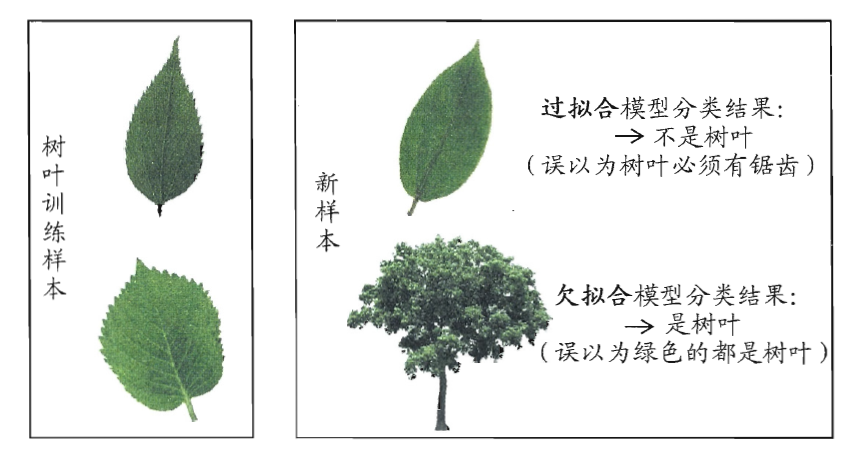
\includegraphics[width=0.8\linewidth]{img/fitting.jpg} 
%  \renewcommand{\figurename}{图} 
% \caption{过拟合、欠拟合的直观类比} 
% %英文标题begin 
% \addtocounter{figure}{-1} \vspace{-5pt} 
% %\SetEnglishCaption 
% \renewcommand{\figurename}{Fig} 
% \caption{Visual analogy of overfitting and underfitting} 
% \renewcommand{\figurename}{图} 
% %英文标题end 
% \label{fig:network-device-influence.png} 
% \end{figure}



 \indent 机器学习模型往往着力于解决的过拟合问题。在实践中往往有多种原因导致过拟合问题的出现。较为常见的情况有,因模型学习能力过于强而导致训练数据集中所包含的非一般特性都被模型学习到。而欠拟合则通常是由于模型复杂度低下和学习能力不足造成,例如在神经网络学习中采取增加模型网络深度和增加训练轮数可以克服欠拟合问题。与之相对的过拟合问题是机器学习面临的核心阻碍,在各类具体的机器学习模型中都有各自机制来应对,但原则上过拟合问题是不可避免的,以上的机制也只能部分的缓解过拟合问题。(周志华, 2016)。\\
 \indent 一般的可以通过实验测试来对机器学习模型的泛化能力进行评估,同时完成对模型参数的选择。故我们需要一个有别于训练数据集(training set)的测试数据集(testing set)。若假设测试数据集中新样本也是从真实事件分布中独立同分布采样而得到,同时测试数据集与训练数据集互斥度越大越佳,这就意味着测试数据集中样本尽量没有出现过在训练过程中。在这种假设下我们可以使用测试数据集的测试误差(testing error)作为模型对于真实泛化能力的估计。机器学习模型对于新样本的分别能力越出众,则其在测试数据集上的误差越小。对于一个包含m个样本的数据集$D=\left\{\left(\boldsymbol{x}_{1}, y_{1}\right),\left(\boldsymbol{x}_{2}, y_{2}\right), \ldots\right.\left(\boldsymbol{x}_{m}, y_{m}\right) \}$,通常从D中适当的分出训练集S和测试集T两个互斥的子集。\\
 \subsection{朴素留出训练方法}
 \indent 常见朴素法通常的做法为直接将全数据集D划分为互斥的两个集合,这两个集合S、T满足,$D=S \cup T, S \cap T=\varnothing$.~即使用训练数据集S上进行模型训练,随后在测试数据集T上进行模型泛化能力评估。这种两数据集的划分思想被称为朴素留出法。\\
 \indent 留出法最核心的问题是需要既要使训练集和测试集分布保持一致性又要使得两个集合足够互斥,这就意味着要尽量避免因为分布带来的问题。如果训练数据集与真实分布不一致,则会导致训练出的模型天然有偏差。这就要求假设在面对分类问题时,使用分层采样的方式在不同类别样本上按比例随机采样,保持住训练集和真实分布的一致性。同时考虑到如果测试数据集与真实分布差异过大,显而易见的会使对模型评估的环节变得没有意义,甚至产生负面指导作用。\\
 \indent 朴素留出方法面临着无法解决两难的困境。一方面如果训练集S太小,则给予机器学习模型的训练信息不足够充分难以训练出优秀的模型。另一方面我们希望使用测试数据集T测试出机器学习模型对于评估原始数据集D的能力,所以就要求测试数据集T不能太小,使其能够拥有足够多的原始数据D集中的信息。这导致了在往往有限的数据量的情况下,两个互斥的测试集和训练集都有数据量要求。这一矛盾在数据量有限的情况下无法调和,经验上选取原始数据量的60\%至90\%作为训练集S,剩余未使用过的数据样本纳入测试集T。\\
 \subsection{交叉验证法}
 \indent 交叉验证法(cross validation)为了解决朴素留出法难以平衡评估稳定性和保真性的问题,将原始数据集D划分为k个大小相似的互斥子集(也称为k折交叉检验),即$D=D_{1} \cup D_{2} \cup \ldots \cup D_{k}, D_{i} \cap D_{j}=\varnothing(i \neq j)$,每个子集都采取分层采样的方式来保证数据分布一致性。此方法如下图所示,每次选取k-1个数据集的合并作为训练集,剩余一个数据集作为测试集。如上述描述数据集选取方式的使得单一训练过程的训练数据量足够大。为了兼顾模型评估的保真性,我们重复进行k次以上操作,每次的验证集都是之前训练过程所不相同的,共训练出不一样的k个模型,这些模型结果的平均值作为整个系统的输出用于评估。\\
 \indent 可以看出在数据集比较大时,训练k个模型的开销是巨大的。所以交叉验证法在改善了朴素留出法性能问题的同时,也面临着速度和精度的取舍。\\
\begin{figure}[!h] 
\centering 
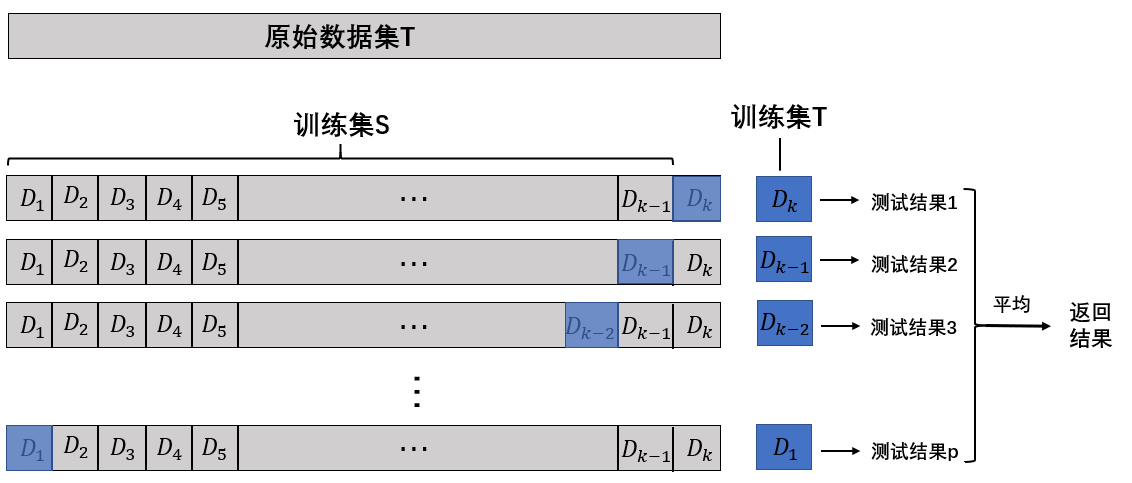
\includegraphics[width=0.95\linewidth]{img/cv.jpg} 
\renewcommand{\figurename}{图} 
\caption{交叉检验示意图} 
%英文标题begin 
\addtocounter{figure}{-1} \vspace{-5pt} 
%\SetEnglishCaption 
\renewcommand{\figurename}{Fig} 
\caption{Cross-validation diagram} 
\renewcommand{\figurename}{图} 
%英文标题end 
\label{fig:network-device-influence.png} 
\end{figure}
\subsection{本次研究模型评估方式}
\indent 若只确定模型大方向的结构,而并未确定例如CNN模型中卷积核大小、池化层池化核移动方式等。在这些具体参数并没固定的情况下,我们需要对模型结构和参数同时进行选择。以上的问题导致了若只使用“训练-测试”的数据划分方式难以对模型泛化能力进行评估。在本文研究中我们结合了朴素留出法和交叉验证法的特点,将所有的地震记录划分为训练集、交叉验证集(cross validation set)和测试集三部分。我们随机将全台站地震记录集的70\%数据划分为训练集,10\%划分为交叉检验集,20\%划分为测试集。区别于以上两种传统模型的数据划分方式,增添了交叉验证集。\\
\indent 考虑到模型训练的时间和效率的限制,不同于交叉检验法的多组模型训练,本次研究采取朴素留出思想只训练出一组模型。使用交叉验证集取代原测试集的作用,结合训练集的数据反复进行模型参数训练,继而对模型训练成果进行评估,最终在完全没有参与过使用的测试集上进行最终的模型选择。\\
\indent 在数据集划分方面更多需要注意的是,由于同一地震事件会有多个台站记录,这些不同台站记录到同一个地震数据间极其相似。这就导致了在划分数据集时不能将这些同属于一个地震事件的单条数据划分到不同数据集合中。否则等同于不同集合之间发生了信息泄露,使得交叉验证集和测试集失去了其存在的意义,所显示出来的泛化能力都是虚假的。\\
\indent 在以一个地震事件为“最小”数据单位的要求下,同时考虑到之前使训练集和测试集分布保持一致性和互斥性的情况下爱,就暴露出了数据总体上数据分布不均和数据量不够的问题,在接下来的第四章中会详细介绍优化和解决方案。\\
	\chapter{总结与展望}
\indent 本文提出了使用机器学习类算法来解决和优化地震紧急预警系统中预估震级部分的思路,设计了两种神经网络模型并成功实现了其中一种。已实现的以NN网络为基础的模型,与已有单台站震级预估算法相比有着更好的效果。通过较为简单的NN模型的实现展示出了此类算法在震级预估问题上的强大优势,同时也为深度学习类的模型探索出了今后研究方向。

\indent 从预估表现来看,与传统的$\mathrm{p}_{\mathrm{d}}$和$\tau_{c}$方法相比,无论对于多事件整体,还是单一事件多台站联合预估NN模型的方差和误差都更小,这意味着预估效果得到提升。但根据单台站所得到的预估结果离散程度仍然很大,测试表明需要5个以上台站才能得到稳定的结果。

\indent 因数据量不足的原因暂时还未实现的CNN模型,是以CNN卷积神经结构为基础深度学习模型。从已有研究结果和其思路来看,无论是使用高通巴特沃斯滤波器的$\mathrm{p}_{\mathrm{d}}$法、还是使用傅里叶变换的$\tau_{c}$法,本质都为对原始地震记录数据使用某种方式的滤波、变换后的某一特征。这对于深度学习CNN网络表达能力是完全能够达到的,并且对于有一定深度CNN网络可期待其得到其他的变换、滤波下的未知特征。将这些特征组合使用,可望得到更为优异的模型。

\indent NN模型中没有使用位置信息,对于正在实现中的CNN模型,在其最后卷积层的输出后引入了台站和震源的经纬信息,这使其可能在区域内获得断层信息、地球介质信息的记录能力,而不是像$\mathrm{p}_{\mathrm{d}}$方法单纯使用震中距。这可能是解决单一台站预估结果离散过大的一种有效途径。

\indent 本文采取了在训练集中对大震级事件过采样的方法,以处理类别不平衡问题。此后还可以继续尝试使用再缩放法结合过采样法,进一步处理和优化天然地震震级分布不均的问题。




    \chapter{总结与展望}
\indent 本文提出了使用机器学习类算法来解决和优化地震紧急预警系统中预估震级部分的思路,设计了两种神经网络模型并成功实现了其中一种。已实现的以NN网络为基础的模型,与已有单台站震级预估算法相比有着更好的效果。通过较为简单的NN模型的实现展示出了此类算法在震级预估问题上的强大优势,同时也为深度学习类的模型探索出了今后研究方向。

\indent 从预估表现来看,与传统的$\mathrm{p}_{\mathrm{d}}$和$\tau_{c}$方法相比,无论对于多事件整体,还是单一事件多台站联合预估NN模型的方差和误差都更小,这意味着预估效果得到提升。但根据单台站所得到的预估结果离散程度仍然很大,测试表明需要5个以上台站才能得到稳定的结果。

\indent 因数据量不足的原因暂时还未实现的CNN模型,是以CNN卷积神经结构为基础深度学习模型。从已有研究结果和其思路来看,无论是使用高通巴特沃斯滤波器的$\mathrm{p}_{\mathrm{d}}$法、还是使用傅里叶变换的$\tau_{c}$法,本质都为对原始地震记录数据使用某种方式的滤波、变换后的某一特征。这对于深度学习CNN网络表达能力是完全能够达到的,并且对于有一定深度CNN网络可期待其得到其他的变换、滤波下的未知特征。将这些特征组合使用,可望得到更为优异的模型。

\indent NN模型中没有使用位置信息,对于正在实现中的CNN模型,在其最后卷积层的输出后引入了台站和震源的经纬信息,这使其可能在区域内获得断层信息、地球介质信息的记录能力,而不是像$\mathrm{p}_{\mathrm{d}}$方法单纯使用震中距。这可能是解决单一台站预估结果离散过大的一种有效途径。

\indent 本文采取了在训练集中对大震级事件过采样的方法,以处理类别不平衡问题。此后还可以继续尝试使用再缩放法结合过采样法,进一步处理和优化天然地震震级分布不均的问题。




            \appendix
\chapter{稀疏矩阵压缩}

\indent 参与破裂过程计算的积分核为稀疏矩阵,在存储的过程中会造成内存的浪费。针对积分核为稀疏矩阵的的情况,我们可以采取一定的矩阵压缩方案。

\section{基本思想}
\indent 在矩阵中,若数值为0的元素数目远远多于非0元素的数目,并且非0元素分布没有规律时,则称该矩阵为稀疏矩阵。因此,基本的想法是只记录稀疏矩阵非零元素的坐标和元素值,通过存储的坐标访问对应的元素值。对于找不到坐标信息的元素时,可直接得到该元素为~0~元素。一个~$4 \times 4$~的2维矩阵~B~为例
$$ B = 
\begin{bmatrix}
   0 & 2 & 0& 0 \\
   4 & 0 & 6 & 0\\
   0 & 8 & 0 & 0\\
   0 & 0 & 0 & 1
  \end{bmatrix} \tag{三维稀疏矩阵}
 $$
 我们记录矩阵B非零元素行列信息和对应的值如\ref{juzhen-yasuo}所示。这样原有的稀疏矩阵被拆分为两个部分存储,一个是非零元素的坐标信息,一个是非零元素的值,则存储空间为非零元素的两倍。假设零元素数目为~$m$~,非零元素为~$n$~。由于~$m>>n$~,因此 ~$2m<<m+n$。这我们实现了稀疏矩阵的压缩存储过程。

\begin{table}
\centering  
\caption{矩阵压缩方案} \label{juzhen-yasuo} 
\begin{tabular}{|c|c|c|c|}
 \hline
行坐标&列坐标& 矩阵值& 矩阵元素\\
 \hline
1 & 2 & 2& $B_{12}$ \\
 \hline
2&1 & 4 &  $B_{21}$\\
 \hline
2 & 3 & 6& $B_{23}$\\
 \hline
3 & 2 & 8& $B_{32}$ \\
 \hline
4 & 4 & 1& $B_{44}$ \\
\hline
\end{tabular}\\
\end{table}


 \section{存在的问题与反思}
 \indent 通过这样的矩阵压缩技术的确能够减小内存的占用,对于第三章中的数值算例一,在破裂过程计算中,积分核存储空间减少了~\%20,然而计算时间却增加了2倍之多。究其原因,我们可以发现,由于采取了压缩技术,在破裂过程的计算中需要添加判断条件来判断积分核的值,由于目前的破裂过程计算采用的是循环计算的方式,因此,时间累积,大大增加了我们的计算时间。因此,对于矩阵压缩,仍然由两个可以改进的方向:1、考虑积分核以矩阵的方式进行破裂过程的计算,这里需要对相应的矩阵计算进行优化。2、目前之考虑了~0~元素的情况,然而实际上,在非零元素中,处于稳定区的那部分稳定值也占据了不少的空间,因此对于稳定值存储的优化也是一个可以考虑的方向。
 
 
 \chapter{公式说明}
 
  在第二章中,公式\ref{con:L311}中各项的详细含义如下,$\Delta = CA-\frac{B^{2}}{4}$,$\Delta_{1}=EA-\frac{BD}{2}$,$\Delta_{2} = \Delta_{1} + (\frac{B^{2}}{2A}-C)F$,$r=(Ax^2+Bx+C)^{1/2} $,$r^{'} = \frac{Ax+\frac{B}{2}}{(Ax^2+Bx+C)^{1/2}}$。而不定积分~$f_{i}$~的表达式如下所示:
        \begin{align}
            f_{1}(A,B,C,D,E) &= \frac{1}{A} \frac{\Delta_{1}}{\Delta}r^{'}-\frac{D}{A} \frac{1}{r}
            \\
            f_{2}(A,B,C,D,E) &= \frac{\Delta_{1}}{\Delta}r^{'}(\frac{2}{3}\frac{1}{\Delta}+\frac{1}{3Ar^{2}})-\frac{D}{3A}\frac{1}{r^{3}}\\
            f_{3}(A,B,C,D,E) &=\frac{\Delta_{1}}{\Delta}r^{'}(\frac{8}{15}\frac{A}{\Delta^{2}}+\frac{4}{15\Delta r^{2}}+\frac{1}{5Ar^{4}})-\frac{D}{5A}\frac{1}{r^{5}} \\
            f_{4}(A,B,C,D,E) &= \frac{\Delta_{2}}{\Delta}r^{'}(\frac{2}{3}\frac{1}{\Delta}+\frac{1}{3Ar^{2}})-\frac{D-\frac{B}{A}F}{3A}\frac{1}{r^{3}}+\frac{F}{A}\frac{r^{'}}{\Delta}\\ \notag
            f_{5}(A,B,C,D,E) &= \frac{\Delta_{2}}{\Delta}r^{'}(\frac{8}{15}\frac{A}{\Delta^{2}}+\frac{4}{15\Delta r^{2}}+\frac{1}{5Ar^{4}})-\frac{D-\frac{B}{A}F}{5A}\frac{1}{r^{5}} + \frac{2}{3}\frac{F}{\Delta^{2}}r^{'} \\ 
            &+ \frac{F}{3A\Delta}\frac{r^{'}}{r^{2}}\\  \notag
        \end{align}
    \indent 此外,记定积分为公式\ref{con:dingjifen},想要确定~$s_1$~与~$s_2$,与它等价的问题是求当 ~$x \in [0,1]$~满足~f(x)<0~的范围。其中~f(x)~为一个二次函数,它的判别式为$\Delta$。 
    \begin{align} \label{con:dingjifen}
        \int_{0}^{1}H(t-r/c)dx=\int_{s_{1}}^{s_{2}} dx
    \end{align}
    
    当$\Delta >0$时,记方程~f(x)=0~的两根为~$r_1$~和~$r_2$~,分类讨论可以得到上下限满足:\\
    1.~$f(0) \le 0 $~,$~f(1)  \le 0$     ~~~~~~~$s_{1} =0$~,~$s_{2} = 1$\\
    2.~$f(0) \le 0 $~,$~f(1)  > 0$     ~~~~~~~$s_{1} =0$~,~$s_{2} = r_{2}$ \\
    3.~$f(0) > 0 $~,$~f(1)  \le 0$~~~~~~~~$s_{1} =r_{1}$~,~$s_{2} = 1$\\
    4.~$f(0) > 0 $~,$~f(1)  > 0$,$0<\displaystyle\frac{(b_{1}-a_{1})^{2} + (b_{2}-a_{2})^{2}}{(b_1 - a_1)(x_1 -b_1)+(b_2-a_2)(x_2-b_2)}<1$~(二次函数对称轴)~~~~~~~$s_{1} =r_{1}$~,~$s_{2} = r_{2}$\\
    5.~其它情况~~~~~~~原积分$  \int_{0}^{1}H(t-r/c)dx = 0$\\
    最后,为了避免混淆,我们约定
    \begin{align} 
         \int_{0}^{1}H(t-r/c_T)dx=\int_{z_{1}}^{z_{2}} dx \label{con:def-sxxian1}\\
          \int_{0}^{1}H(t-r/c_L)dx=\int_{y_{1}}^{y_{2}} dx \label{con:def-sxxian2}
    \end{align} 
    

    
	% 结论。
	% Copyright (c) 2008-2009 solvethis
% Copyright (c) 2010-2011 Casper Ti. Vector
% Public domain.




	\begin{appendix}
		% 参考文献。
		\nocite{*}
		\bibliography{ref/pkuthss.bib}
		
	\end{appendix}

	% 以下为正文之后的部分。
	\backmatter

	% 致谢。
	% Copyright (c) 2008-2009 solvethis
% Copyright (c) 2010-2011 Casper Ti. Vector
% Public domain.

\chapter{致谢}

\indent 感谢张海明老师两年来对我的教诲和关怀。从大三伊始,我便参加了张海明老师的组会。在这两年以来,张老师在学习和研究中给予了我诸多指导,让我能够有机会了解和接触到学术研究工作。无论是在本文的研究中,还是在本科生科研的研究中,张老师都花费了巨大的心血来指导我的工作。在学术上,张老师秉承严谨的作风。对于研究,无论是在实质内容上,还是展示的形式,张老师对于我们都是严格要求。因此,虽然现在的学术研究水平仍然非常有限,但是在张老师的严格要求之下,也能看到自己的进步。除此之外,张老师对于自我价值的坚持,和对于学术最本质的热爱也让人敬佩不已。\\
\indent 此外,还要感谢研究小组的冯禧师兄,和钱峰师兄。在和他们讨论的过程中给我很多思路和灵感,同时在该论文完成的过程中,两位师兄也给予了诸多的建议。同时,师兄们对于学术和知识的追求以及对于研究工作认真、刻苦的精神,时刻激励着我。\\
\indent 感谢本科期间所有的老师。四年来是你们让我从一个懵懂的少年成长为了一位具备一定的基础知识,具有初步科研能力的成熟大学生。在燕园4年的课堂上,我不仅得到了知识的提升,更是能力,认知,思想的进步。\\
\indent 感谢我的室友卢思奇,姜鹏飞,龚旭日。大学四年,无论是在学习上,还是在生活中,都受到了他们的诸多关照。感谢向直柳大学四年的陪伴,在我困惑迷茫之时给予了我很多安慰。感谢各位同学,朋友在大学四年的陪伴以及给予我的帮助。\\
\indent 最后要感谢我的父母和家人。是你们对我全力的理解和支持让我能够全力以赴在这求学之旅上前行。
	% 原创性声明和使用授权说明。
	% Copyright (c) 2008-2009 solvethis
% Copyright (c) 2010-2011 Casper Ti. Vector
% All rights reserved.
%
% Redistribution and use in source and binary forms, with or without
% modification, are permitted provided that the following conditions are
% met:
%
% * Redistributions of source code must retain the above copyright notice,
%   this list of conditions and the following disclaimer.
% * Redistributions in binary form must reproduce the above copyright
%   notice, this list of conditions and the following disclaimer in the
%   documentation and/or other materials provided with the distribution.
% * Neither the name of Peking University nor the names of its contributors
%   may be used to endorse or promote products derived from this software
%   without specific prior written permission.
% 
% THIS SOFTWARE IS PROVIDED BY THE COPYRIGHT HOLDERS AND CONTRIBUTORS "AS
% IS" AND ANY EXPRESS OR IMPLIED WARRANTIES, INCLUDING, BUT NOT LIMITED TO,
% THE IMPLIED WARRANTIES OF MERCHANTABILITY AND FITNESS FOR A PARTICULAR
% PURPOSE ARE DISCLAIMED. IN NO EVENT SHALL THE COPYRIGHT HOLDER OR
% CONTRIBUTORS BE LIABLE FOR ANY DIRECT, INDIRECT, INCIDENTAL, SPECIAL,
% EXEMPLARY, OR CONSEQUENTIAL DAMAGES (INCLUDING, BUT NOT LIMITED TO,
% PROCUREMENT OF SUBSTITUTE GOODS OR SERVICES; LOSS OF USE, DATA, OR
% PROFITS; OR BUSINESS INTERRUPTION) HOWEVER CAUSED AND ON ANY THEORY OF
% LIABILITY, WHETHER IN CONTRACT, STRICT LIABILITY, OR TORT (INCLUDING
% NEGLIGENCE OR OTHERWISE) ARISING IN ANY WAY OUT OF THE USE OF THIS
% SOFTWARE, EVEN IF ADVISED OF THE POSSIBILITY OF SUCH DAMAGE.

% 原创性声明和使用授权说明页不需要装订到论文中,故不显示页码。
\cleardoublepage\pagestyle{empty}
{
	\linespread{1.5}\selectfont
	\section*{北京大学学位论文原创性声明和使用授权说明}

	\vfill
	\section*{原创性声明}

	本人郑重声明:
	所呈交的学位论文,是本人在导师的指导下,独立进行研究工作所取得的成果。
	除文中已经注明引用的内容外,
	本论文不含任何其他个人或集体已经发表或撰写过的作品或成果。
	对本文的研究做出重要贡献的个人和集体,均已在文中以明确方式标明。
	本声明的法律结果由本人承担。
	\vspace{2.5em}\par
	\rightline
	{%
		论文作者签名:\hspace{5em}%
		日期:\hspace{2em}2018年\hspace{2em}6月\hspace{2em}12日%
	}

	\vfill
	\section*{学位论文使用授权说明}
	\vspace{-1em}\par
	\centerline{\zihao{-4}(必须装订在提交学校图书馆的印刷本)}
	\vspace{1em}\par

	本人完全了解北京大学关于收集、保存、使用学位论文的规定,即:
	\begin{itemize}
		\item 按照学校要求提交学位论文的印刷本和电子版本;
		\item 学校有权保存学位论文的印刷本和电子版,
			并提供目录检索与阅览服务,在校园网上提供服务;
		\item 学校可以采用影印、缩印、数字化或其它复制手段保存论文;
		\item 因某种特殊原因需要延迟发布学位论文电子版,
			授权学校在 $\square$\nobreakspace{}一年 / %
			$\square$\nobreakspace{}两年 / %
			$\square$\nobreakspace{}三年以后在校园网上全文发布。
	\end{itemize}
	\par(保密论文在解密后遵守此规定)
	\vspace{2.5em}\par
	\rightline
	{%
		论文作者签名:\hspace{5em}导师签名:\hspace{5em}%
		日期:\hspace{2em}2018年\hspace{2em}6月\hspace{2em}12日%
	}
	\par
}


\end{document}

